\subsection{V2}
Video \textit{V2} is recorded at 29 fps. Only the cars driving from the left to the right are detected and tracked. In
the following
experiments
frames 83-109 of the
video \textit{V2} are
analyzed.
\subsection{V2 -- GM-PHD with the constant detection probability}
The measurements for the GM-PHD filter with the constant detection probability are obtained by the YOLO object detection
model. The parameters' values are displayed in Table \ref{tab:E1-V2-S0}.
\begin{table}[!h]
    \centering
    \begin{tabular}{|c|c|c|c|c|c|}
        \hline
        $P_{D}$ & $P$ & $\sigma_{\upsilon}$ & $\sigma_{\epsilon}$ & $T_p$ & $T_{YOLO}$ \\ \noalign{\hrule height 1.5pt}
        0.9 & $\diag(100,100,100,100)$ & 0.1 & 30 & 0.1 & 0.3\\
        \hline
    \end{tabular}
    \caption{The parameter settings for Experiment E1-V2 with the constant detection probability.}
    \label{tab:E1-V2-S0}
\end{table}

Figure \ref{fig:E1-V2-S0} displays the performance of the GM-PHD filter with the constant detection probability.
\begin{itemize}
    \item \textbf{\ref{fig:E1-V2-S0:01}:} The sequence begins with the frame number 83, wherein four targets have
    already been initialized and successfully detected.
    \item \textbf{\ref{fig:E1-V2-S0:02}:} Notably, the objects appear relatively small in comparison to the overall
    frame size. This size discrepancy contributes to a phenomenon where targets in a close proximity share
    measurements, resulting in the appearance of additional targets in the scene.
    \item \textbf{\ref{fig:E1-V2-S0:03}:} Despite the YOLO model failing to detect the fourth car, the target persists within the tracking system.
    \item \textbf{\ref{fig:E1-V2-S0:04}:} The previously undetected car is successfully identified once more, and
    the tracking of the target continues. Additionally, another car approaches the spawning point.
    \item \textbf{\ref{fig:E1-V2-S0:05}:} Regrettably, the car within the spawning area remains undetected and
    has not survived, probably
    due to its weight being insufficient to ensure survival. Concurrently, the first car exits the scene.
    \item \textbf{\ref{fig:E1-V2-S0:06}:} Subsequently, the car at the spawning point is detected once again and remains sufficiently close to be initialized as a target. The scene concludes with four true objects and four accurately tracked targets.
\end{itemize}


The GM-PHD filter with the constant detection probability is accurate in scenarios, where the object detector does not
miss detections regularly. Figure \ref{gr:E1-V2-S0} shows that the number of displayed targets is close enough
to the true count. Even false detections created by YOLO did not mislead the filter.


\begin{figure}[H]
    \centering
    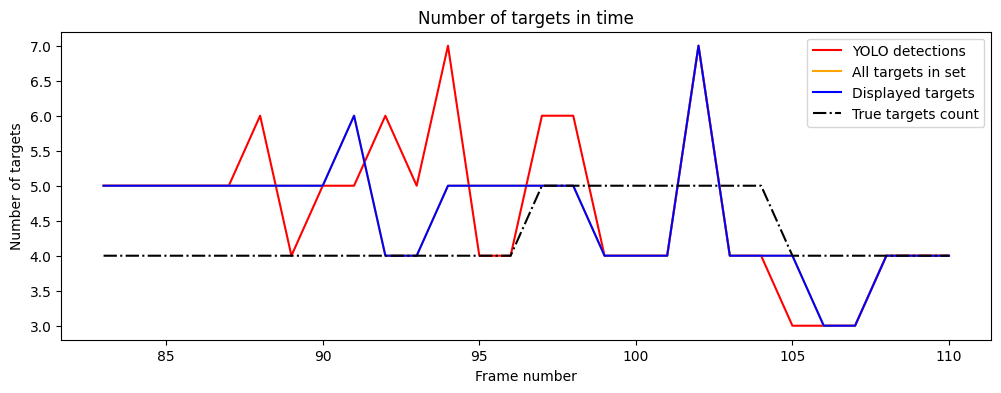
\includegraphics[width=\linewidth]{../../../experiments/E1/V2/noPd/staticPd_det}
    \caption{Development chart of the number of detected targets, targets in the filter's queue, displayed targets
    and the
    true
    targets' count.}
    \label{gr:E1-V2-S0}
\end{figure}

\begin{figure}[H]
    \centering
    \begin{subfigure}{0.48\textwidth}
        \centering
        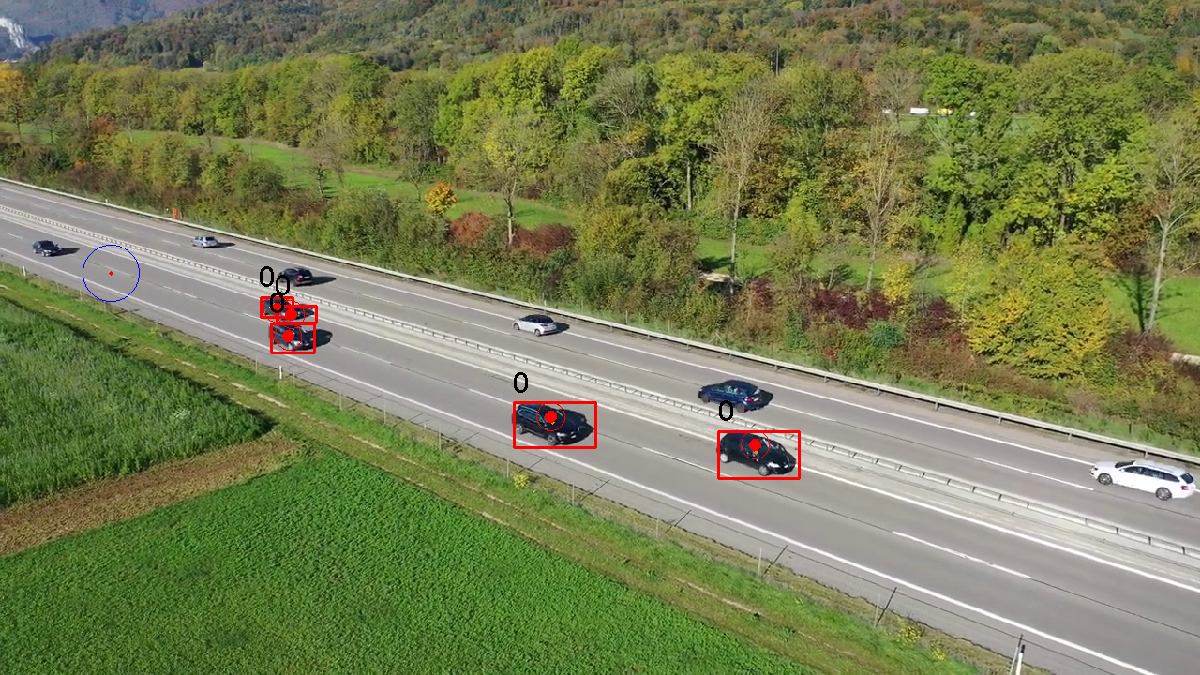
\includegraphics[width=\linewidth]{../../../experiments/E1/V2/noPd/83}
        \caption{Frame number: 83.}
        \label{fig:E1-V2-S0:01}
    \end{subfigure}
    \begin{subfigure}{0.48\textwidth}
        \centering
        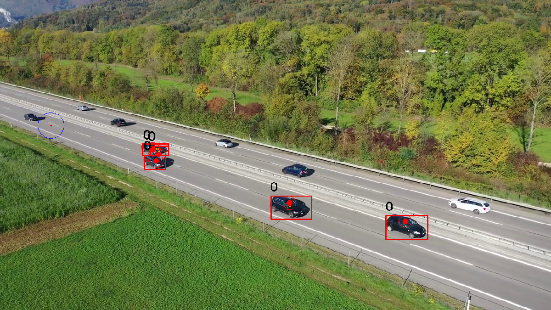
\includegraphics[width=\linewidth]{../../../experiments/E1/V2/noPd/90}
        \caption{Frame number: 90.}
        \label{fig:E1-V2-S0:02}
    \end{subfigure}
    \\
    \begin{subfigure}{0.48\textwidth}
        \centering
        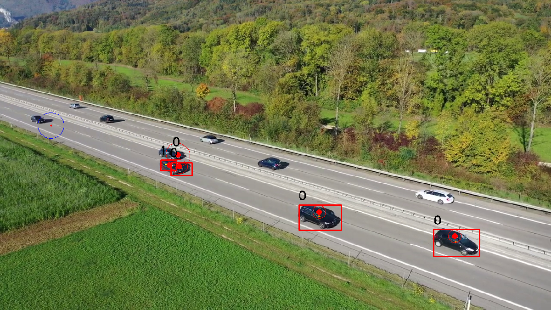
\includegraphics[width=\linewidth]{../../../experiments/E1/V2/noPd/95}
        \caption{Frame number: 95.}
        \label{fig:E1-V2-S0:03}
    \end{subfigure}
    \begin{subfigure}{0.48\textwidth}
        \centering
        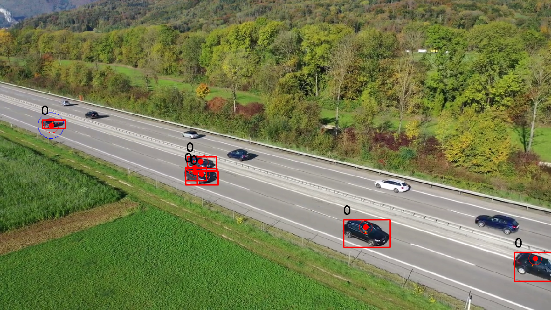
\includegraphics[width=\linewidth]{../../../experiments/E1/V2/noPd/102}
        \caption{Frame number: 102.}
        \label{fig:E1-V2-S0:04}
    \end{subfigure}
    \\
    \begin{subfigure}{0.48\textwidth}
        \centering
        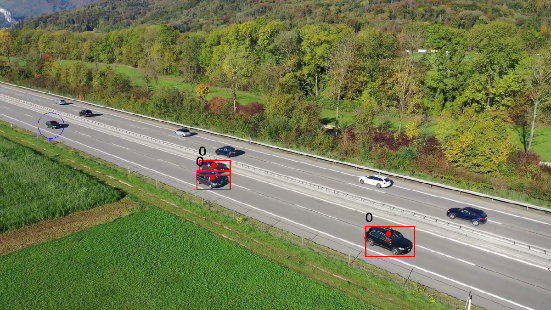
\includegraphics[width=\linewidth]{../../../experiments/E1/V2/noPd/105}
        \caption{Frame number: 105.}
        \label{fig:E1-V2-S0:05}
    \end{subfigure}
    \begin{subfigure}{0.48\textwidth}
        \centering
        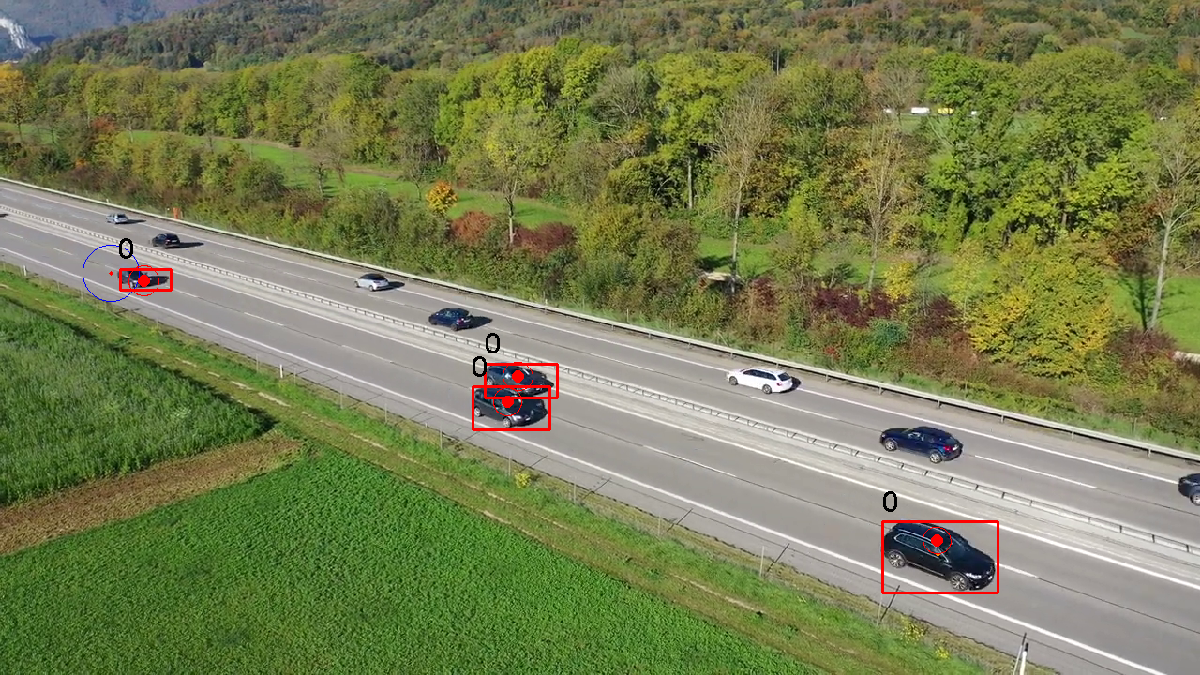
\includegraphics[width=\linewidth]{../../../experiments/E1/V2/noPd/110}
        \caption{Frame number: 110.}
        \label{fig:E1-V2-S0:06}
    \end{subfigure}
    \caption{Image sequence of tracked objects using the GM-PHD filter with the constant detection probability.}
    \label{fig:E1-V2-S0}
\end{figure}


\subsection{V2 -- GM-PHD with the dynamic detection probability}
Experiments carried out on the video \textit{V2} using the GM-PHD filter with the dynamic detection probability and
different
settings
are
demonstrated in following sections.
\subsubsection{S1 -- YOLO + YOLO}
This experiment uses settings \textit{S1}, where the YOLO model provides both object detection bboxes and
segmentation masks.
The parameter settings are shown in Table \ref{tab:E1-V2-S1}.
\begin{table}[H]
    \centering
    \begin{tabular}{|c|c|c|c|c|c|c|c|c|}
        \hline
        $P_{D,k}(x)$ & $P$ & $\sigma_{\upsilon}$ & $\sigma_{\epsilon}$ & $T_H$ & $T_d$ & $T_p$ & $T_l$ & $T_{YOLO}$ \\ \noalign{\hrule
        height 1.5pt}
        0.3 & $\diag(600,600,600,600)$ & 0.1 & 30 & 1 & 3 & 0.1 & 0.01 & 0.3\\
        \hline
    \end{tabular}
    \caption{The parameter settings for Experiment E1-V2-S1 with the dynamic detection probability.}
    \label{tab:E1-V2-S1}
\end{table}

Figure \ref{fig:E1-V2-S1} shows the performance of the GM-PHD filter with the dynamic detection probability with settings \textit{S1}.
\begin{itemize}
    \item \textbf{\ref{fig:E1-V2-S1:01}:} Analogously to the previous analysis, four targets have surpassed the
    spawning point and are tracked by the GM-PHD filter. The targets' presence in the close proximity results in an
    additional false targets' existence.
    \item \textbf{\ref{fig:E1-V2-S1:02}:} The problem of targets' neighboring persists.
    \item \textbf{\ref{fig:E1-V2-S1:03}:} Moreover, the YOLO model classifies the targets' shadows as another cars,
    causing the initialization of extra targets.
    \item \textbf{\ref{fig:E1-V2-S1:04}:} A new car crosses the spawning point, yet the YOLO model fails to detect it.
    \item \textbf{\ref{fig:E1-V2-S1:05}:} The new car has been previously detected and
    initialized. The two
    neighbouring cars still generate additional false targets.
    \item \textbf{\ref{fig:E1-V2-S1:06}:} Finally, there appear only two targets representing the two cars. The other
    two
    cars are tracked properly.
\end{itemize}

Figure \ref{gr:E1-V2-S1} depicts a similar performance of the GM-PHD filter with the dynamic detection probability as
the GM-PHD filter with the constant detection probability. The number of displayed targets exceeds the true number of
targets due to already presented reasons.


The improved ability of the target's survival resulted in a slightly decreased the overall tracking performance. The
YOLO model
has been able to detect tracked objects flawlessly, which leads to needlessness of the dynamic detection
probability
and modified pruning method enabling enhanced targets' ability to survive.

However, the goal of this experiment is to examine the tracking capability of the GM-PHD filter with the proposed
dynamic
detection probability in common flawless scenarios. This experiment verifies the method to be sufficient.

\begin{figure}[H]
    \centering
    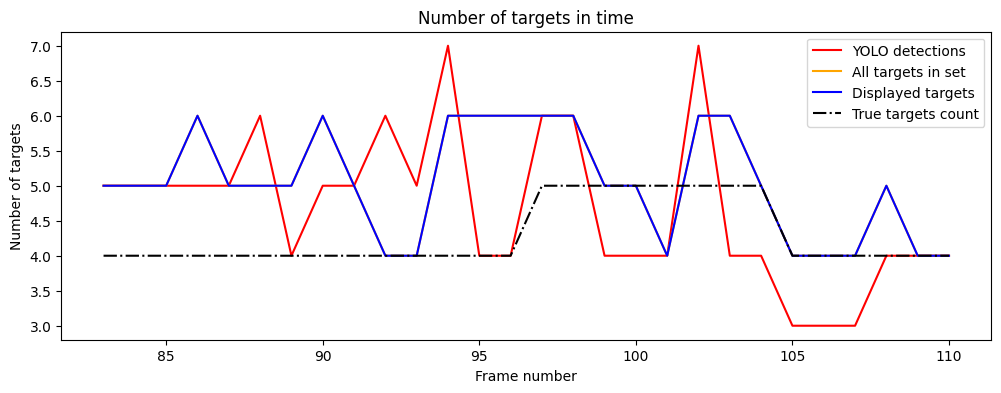
\includegraphics[width=\linewidth]{../../../experiments/E1/V2/YOLO/yolo_det}
    \caption{Development chart of the number of detected targets, targets in the filter's queue, displayed targets
    and the
    true targets' count.}
    \label{gr:E1-V2-S1}
\end{figure}

\begin{figure}[H]
    \centering
    \begin{subfigure}{0.48\textwidth}
        \centering
        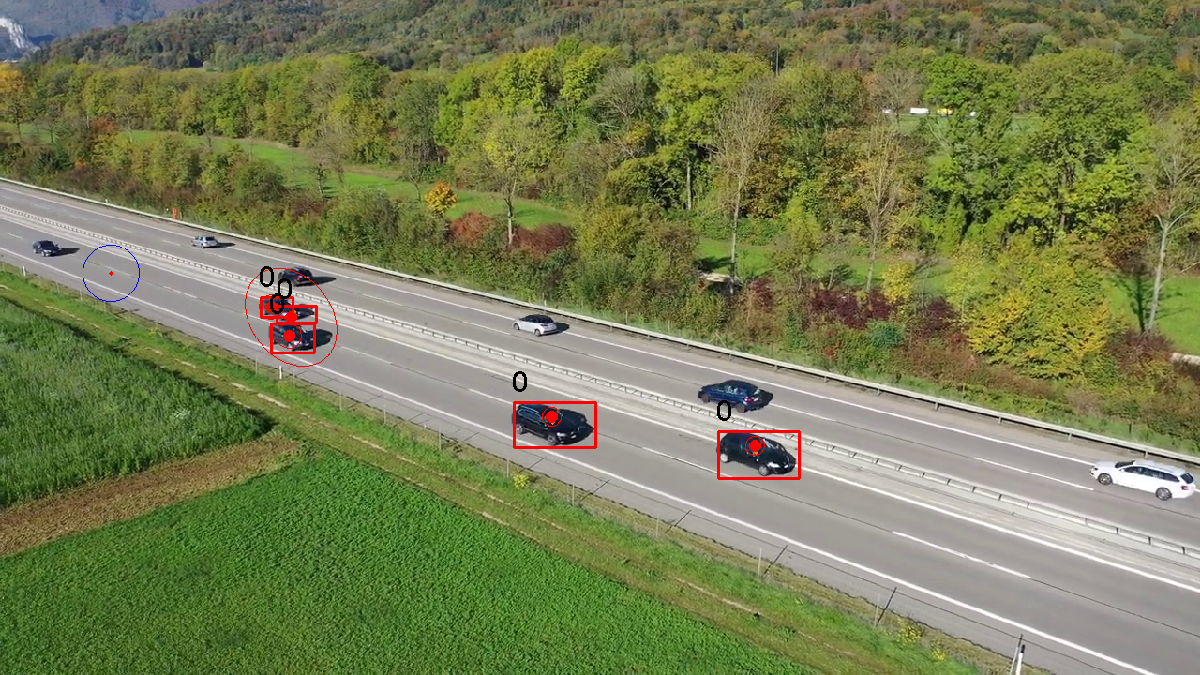
\includegraphics[width=\linewidth]{../../../experiments/E1/V2/YOLO/83}
        \caption{Frame number: 83.}
        \label{fig:E1-V2-S1:01}
    \end{subfigure}
    \begin{subfigure}{0.48\textwidth}
        \centering
        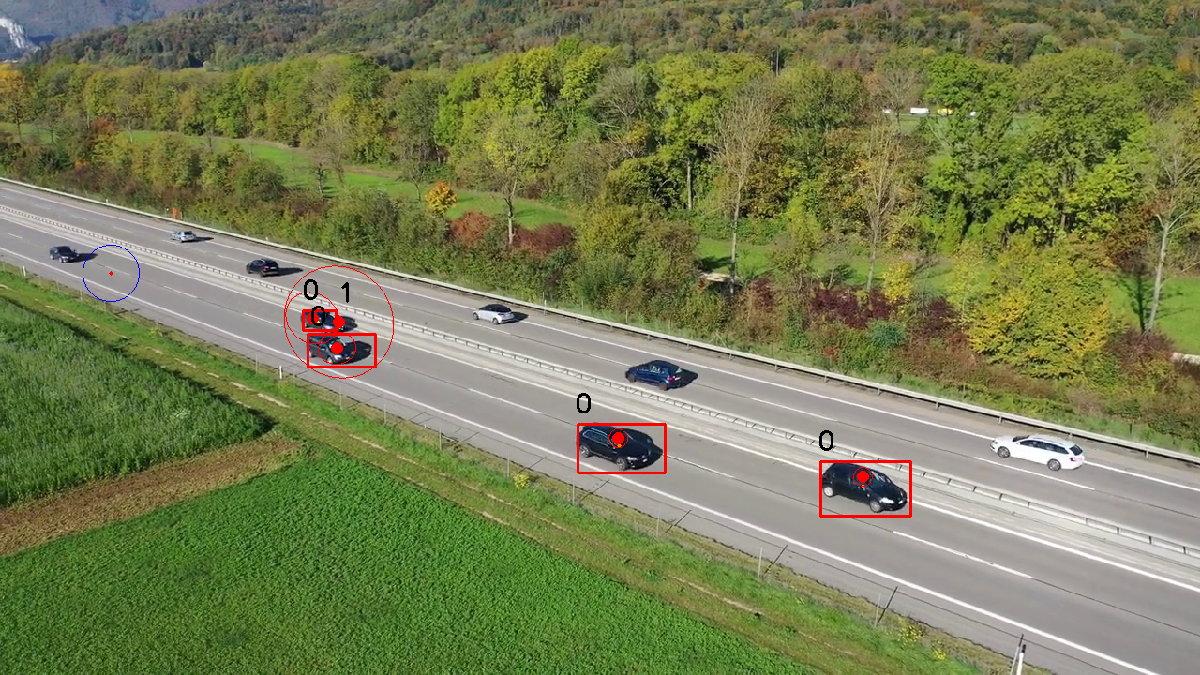
\includegraphics[width=\linewidth]{../../../experiments/E1/V2/YOLO/89}
        \caption{Frame number: 89.}
        \label{fig:E1-V2-S1:02}
    \end{subfigure}
    \\
    \begin{subfigure}{0.48\textwidth}
        \centering
        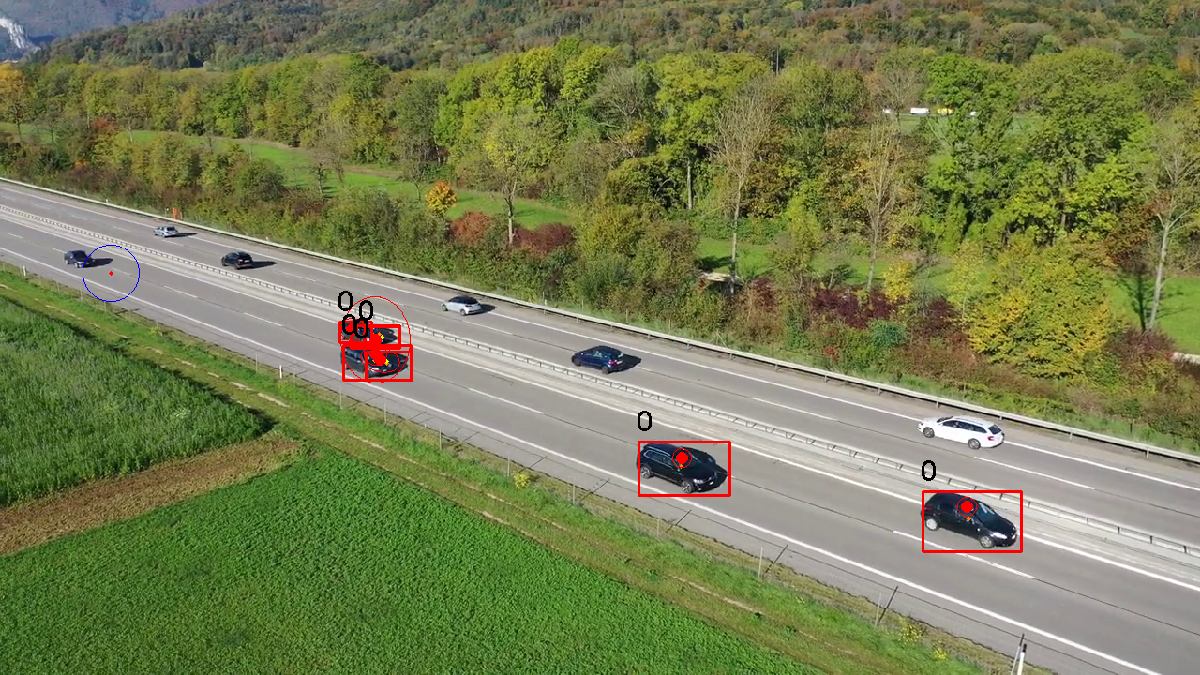
\includegraphics[width=\linewidth]{../../../experiments/E1/V2/YOLO/94}
        \caption{Frame number: 94.}
        \label{fig:E1-V2-S1:03}
    \end{subfigure}
    \begin{subfigure}{0.48\textwidth}
        \centering
        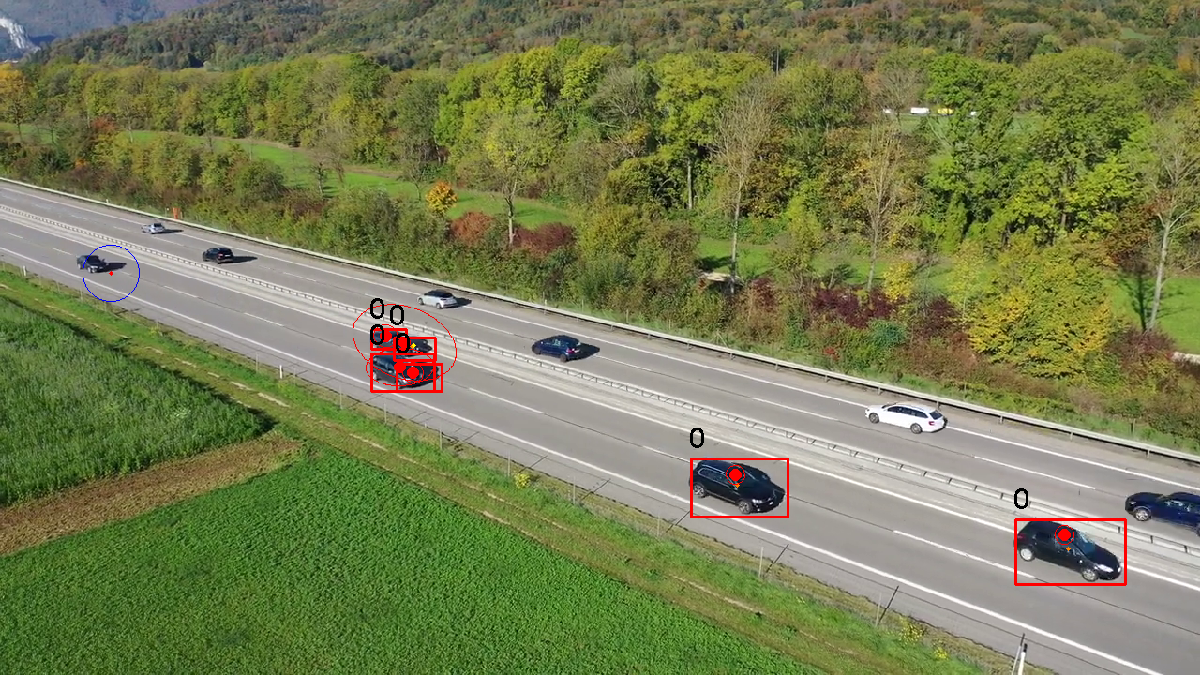
\includegraphics[width=\linewidth]{../../../experiments/E1/V2/YOLO/98}
        \caption{Frame number: 98.}
        \label{fig:E1-V2-S1:04}
    \end{subfigure}
    \\
    \begin{subfigure}{0.48\textwidth}
        \centering
        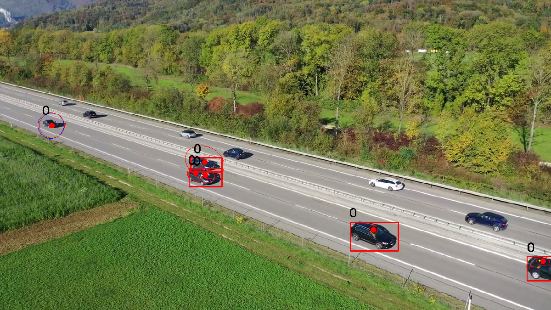
\includegraphics[width=\linewidth]{../../../experiments/E1/V2/YOLO/103}
        \caption{Frame number: 103.}
        \label{fig:E1-V2-S1:05}
    \end{subfigure}
    \begin{subfigure}{0.48\textwidth}
        \centering
        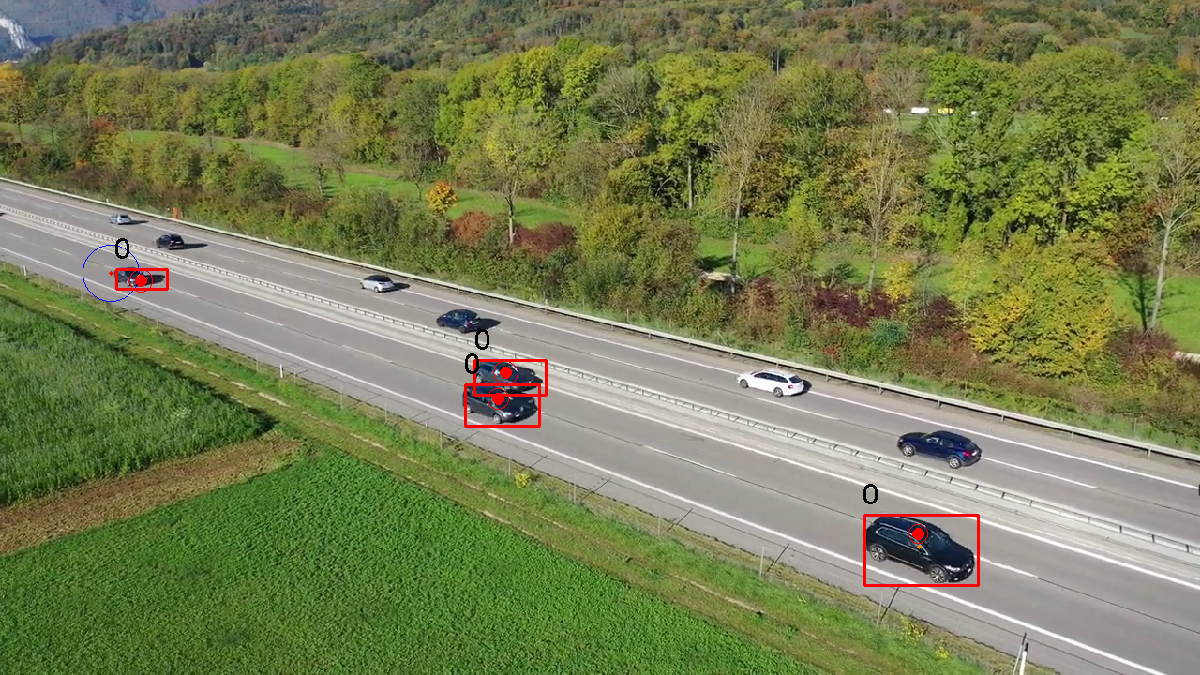
\includegraphics[width=\linewidth]{../../../experiments/E1/V2/YOLO/109}
        \caption{Frame number: 109.}
        \label{fig:E1-V2-S1:06}
    \end{subfigure}
    \caption{Image sequence of tracked objects using the GM-PHD filter with the dynamic detection probability and YOLO
    only.}
    \label{fig:E1-V2-S1}
\end{figure}





\subsubsection{S2 -- YOLO + SAM}
As in experiment \textit{E1}, the next settings employs \textit{S2} with the YOLO object detector and the SAM
segmentation model.
All parameters are included in Table \ref{tab:E1-V2-S2}.
\begin{table}[H]
    \centering
    \begin{tabular}{|c|c|c|c|c|c|c|c|c|}
        \hline
        $P_{D,k}(x)$ & $P$ & $\sigma_{\upsilon}$ & $\sigma_{\epsilon}$ & $T_H$ & $T_d$ & $T_p$ & $T_l$ & $T_{YOLO}$ \\ \noalign{\hrule
        height 1.5pt}
        0.3 & $\diag(100,100,100,100)$ & 0.1 & 30 & 1 & 3 & 0.1 & 0.01 & 0.3\\
        \hline
    \end{tabular}
    \caption{The parameter settings for Experiment E1-V2-S2 with the dynamic detection probability.}
    \label{tab:E1-V2-S2}
\end{table}


The situation resembles the situation with settings \textit{S1}. Four targets occur in Figure \ref{fig:E1-V2-S2:01}.
They continue in their path while all targets are tracked successfully with one exception. No additional targets appear
in the subsequent frames. The YOLO model detects a car's shadow and clasifies it as an another car, which makes
the added target in Figure \ref{fig:E1-V2-S2:03}. Due to the merging step, this false target does not survive to the subsequent
frames. A new car is initialized in Figure \ref{fig:E1-V2-S2:04}. All targets are tracked in the
last frames.

The number of displayed targets is close to the true number of targets in Figure
\ref{gr:E1-V2-S2}. The number of
detected targets exceeds the number of true targets for majority of the time, due to the presence of false
detections.

Settings \textit{S2} exhibit a slight improvement over settings \textit{S1}, which is reflected in the reduced error
between the number of displayed targets and the true count.

\begin{figure}[H]
    \centering
    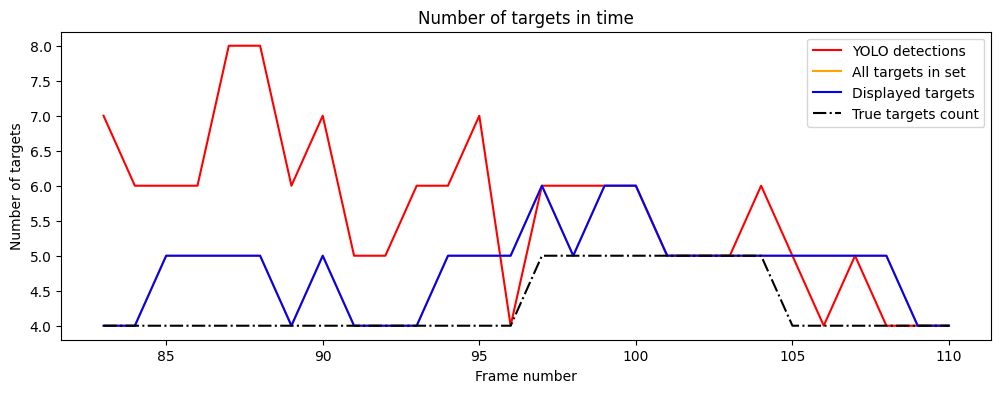
\includegraphics[width=\linewidth]{../../../experiments/E1/V2/SAM/sam_det}
    \caption{Development chart of the number of detected targets, targets in the filter's queue, displayed targets and
    true targets' count.}
    \label{gr:E1-V2-S2}
\end{figure}

\begin{figure}[H]
    \centering
    \begin{subfigure}{0.48\textwidth}
        \centering
        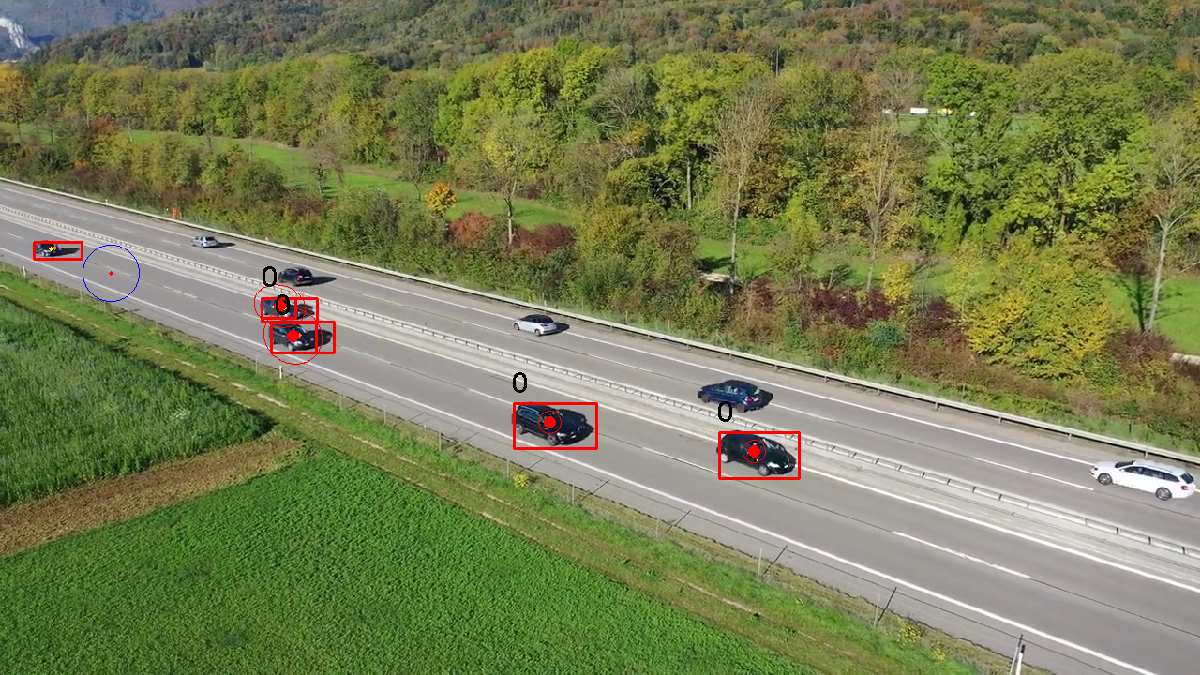
\includegraphics[width=\linewidth]{../../../experiments/E1/V2/SAM/83}
        \caption{Frame number: 83.}
        \label{fig:E1-V2-S2:01}
    \end{subfigure}
    \begin{subfigure}{0.48\textwidth}
        \centering
        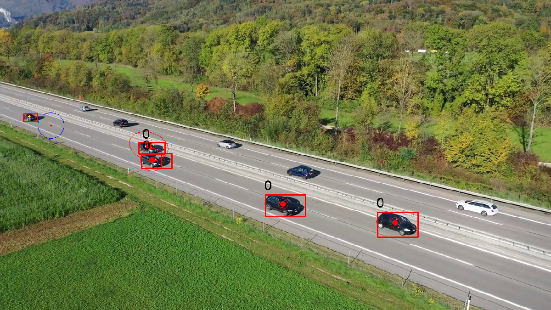
\includegraphics[width=\linewidth]{../../../experiments/E1/V2/SAM/89}
        \caption{Frame number: 89.}
        \label{fig:E1-V2-S2:02}
    \end{subfigure}
    \\
    \begin{subfigure}{0.48\textwidth}
        \centering
        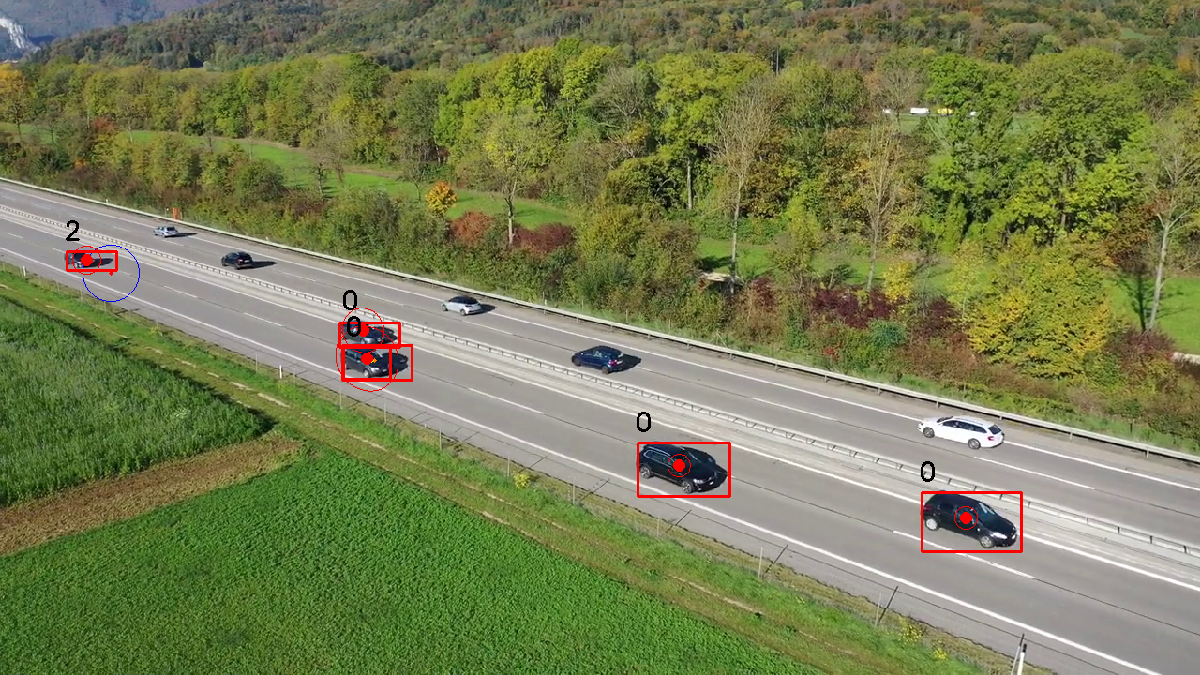
\includegraphics[width=\linewidth]{../../../experiments/E1/V2/SAM/94}
        \caption{Frame number: 94.}
        \label{fig:E1-V2-S2:03}
    \end{subfigure}
    \begin{subfigure}{0.48\textwidth}
        \centering
        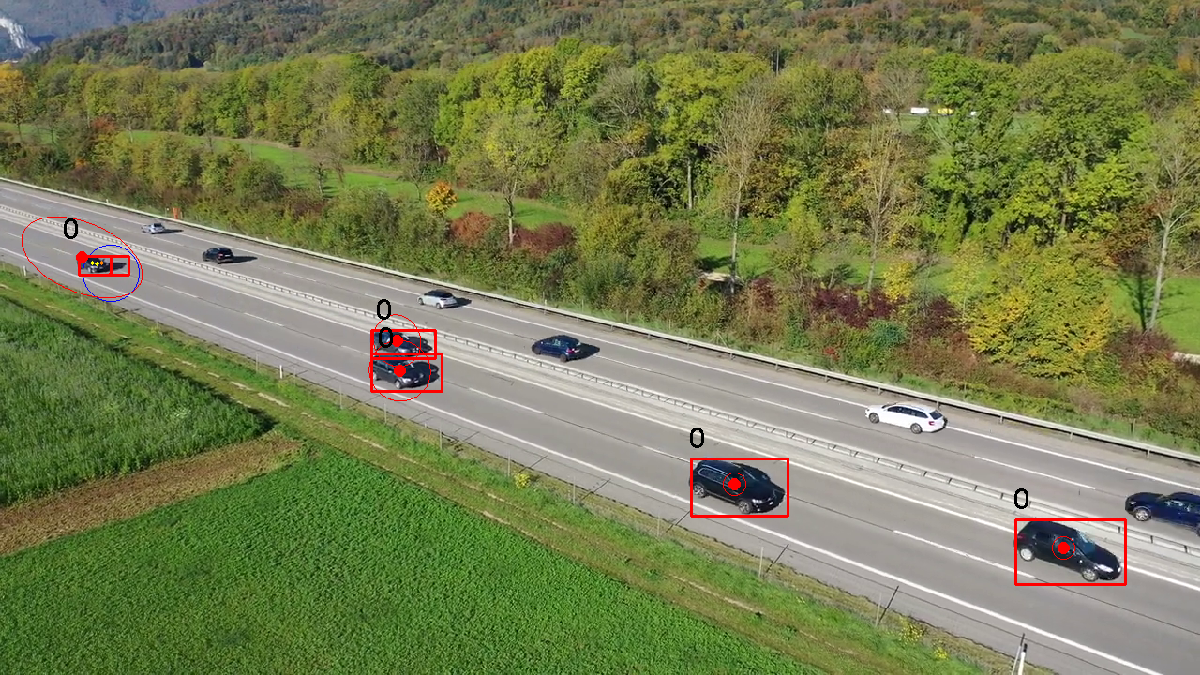
\includegraphics[width=\linewidth]{../../../experiments/E1/V2/SAM/98}
        \caption{Frame number: 98.}
        \label{fig:E1-V2-S2:04}
    \end{subfigure}
    \\
    \begin{subfigure}{0.48\textwidth}
        \centering
        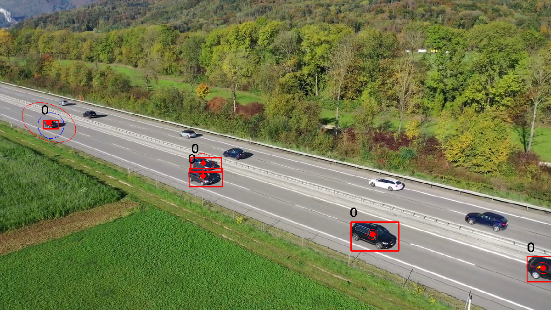
\includegraphics[width=\linewidth]{../../../experiments/E1/V2/SAM/103}
        \caption{Frame number: 103.}
        \label{fig:E1-V2-S2:05}
    \end{subfigure}
    \begin{subfigure}{0.48\textwidth}
        \centering
        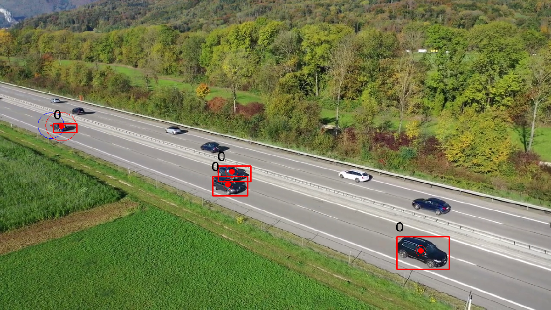
\includegraphics[width=\linewidth]{../../../experiments/E1/V2/SAM/109}
        \caption{Frame number: 109.}
        \label{fig:E1-V2-S2:06}
    \end{subfigure}
    \caption{Image sequence of tracked objects using the GM-PHD filter with the dynamic detection probability, the YOLO
    object detector and the SAM image segmentation model.}
    \label{fig:E1-V2-S2}
\end{figure}


\subsubsection{S3 -- Grounded SAM}
The combination of Grounding DINO and SAM is tested using the video \textit{V2} as well. Used parameteres are given in
Table \ref{tab:E1-V2-S3}.
\begin{table}[H]
    \centering
    \begin{tabular}{|c|c|c|c|c|c|c|c|c|c|}
        \hline
        $P_{D,k}(x)$ & $P$ & $\sigma_{\upsilon}$ & $\sigma_{\epsilon}$ & $T_H$ & $T_d$ & $T_p$ & $T_l$ & $T_{text}$ & $T_{bbox}$\\ \noalign{\hrule
        height 1.5pt}
        0.3 & $\diag(100,100,100,100)$ & 0.1 & 30 & 1 & 3 & 0.1 & 0.01 & 0.3 & 0.3\\
        \hline
    \end{tabular}
    \caption{The parameter settings for Experiment E1-V2-S3 with the dynamic detection probability.}
    \label{tab:E1-V2-S3}
\end{table}

Figure \ref{fig:E1-V2-S3} reveals a better object detection. As a result, the tracking of objects is more precise than
in the other settings.
\begin{itemize}
    \item \textbf{\ref{fig:E1-V2-S3:01}:} Starting with four tracked targets in the frame no. 83.
    \item \textbf{\ref{fig:E1-V2-S3:02}:} As in Experiment E1-V1, the motion and observation noise covariances
    seem to be too large for this scenario. The third and the fourth car's measurement reaches the validation region of
    each other. This situation creates new undesired targets.
    \item \textbf{\ref{fig:E1-V2-S3:03}:} The exact same situation happens in this frame.
    \item \textbf{\ref{fig:E1-V2-S3:04}:} Another car reaches the spawning point.
    \item \textbf{\ref{fig:E1-V2-S3:05}:} Five targets appear in the scene, all of them correctly tracked.
    \item \textbf{\ref{fig:E1-V2-S3:06}:} The scenario ends with four properly detected and tracked objects.
\end{itemize}

Even though the two cars driving side by side cause the filter with given parameters a few modest problems, the merging
and
the pruning steps can usually deal with such situations, as seen in Figure \ref{gr:E1-V2-S3}. The line
showing
the number of displayed targets almost copies the line showing the true counts. The graph also shows the problem of
two neighbouring targets and the problem of false detections. The peaks in the red line show these false detections,
the filter remains unaffected and holds the true number of targets.


As in Experiment \textit{E1-V1}, this setting outperform the other settings variations. Moreover, due to the more
precise
object detection, the filter is able to deal with problems such as two targets appearing in the same neighbourhood or
false
detections. However, settings \textit{S3} is very sensitive to motion and observation noise parametrization, thus
these covariance matrices have to be set carefully.

\begin{figure}[H]
    \centering
    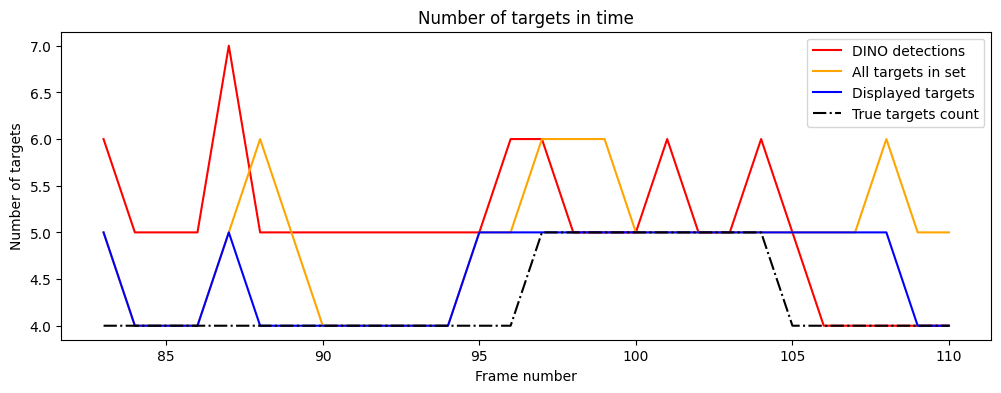
\includegraphics[width=\linewidth]{../../../experiments/E1/V2/DINO/dino_det}
    \caption{Development chart of the number of detected targets, targets in the filter's queue, displayed targets and
    true targets' count.}
    \label{gr:E1-V2-S3}
\end{figure}

\begin{figure}[H]
    \centering
    \begin{subfigure}{0.48\textwidth}
        \centering
        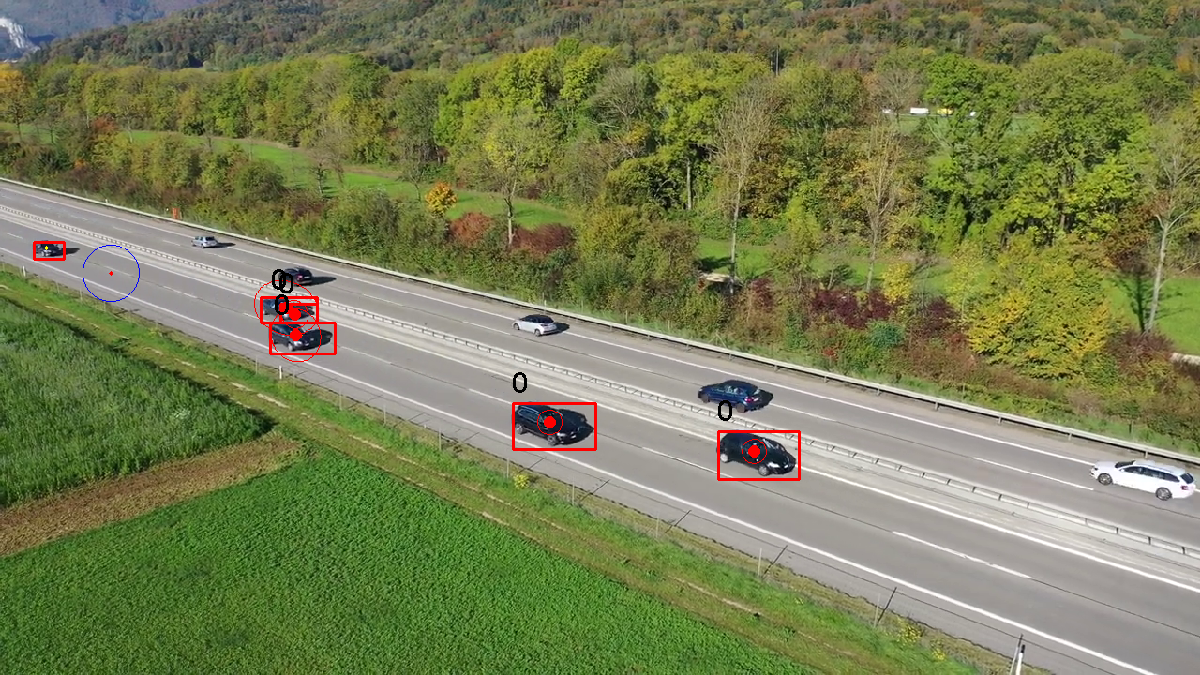
\includegraphics[width=\linewidth]{../../../experiments/E1/V2/DINO/83}
        \caption{Frame number: 83.}
        \label{fig:E1-V2-S3:01}
    \end{subfigure}
    \begin{subfigure}{0.48\textwidth}
        \centering
        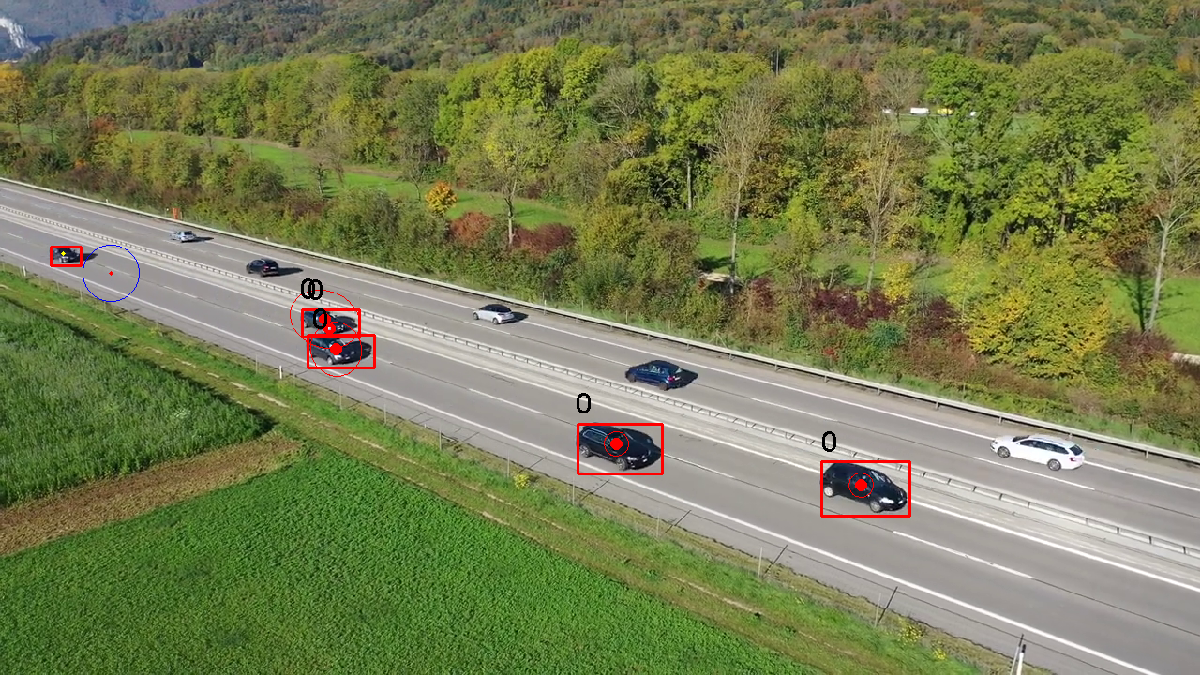
\includegraphics[width=\linewidth]{../../../experiments/E1/V2/DINO/89}
        \caption{Frame number: 89.}
        \label{fig:E1-V2-S3:02}
    \end{subfigure}
    \\
    \begin{subfigure}{0.48\textwidth}
        \centering
        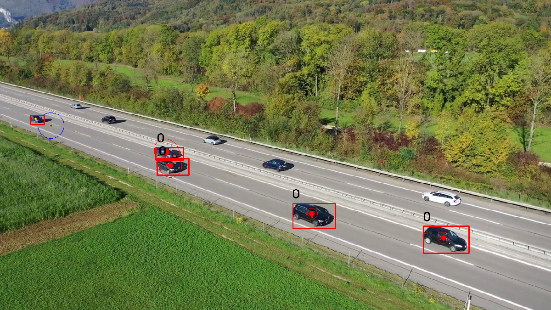
\includegraphics[width=\linewidth]{../../../experiments/E1/V2/DINO/94}
        \caption{Frame number: 94.}
        \label{fig:E1-V2-S3:03}
    \end{subfigure}
    \begin{subfigure}{0.48\textwidth}
        \centering
        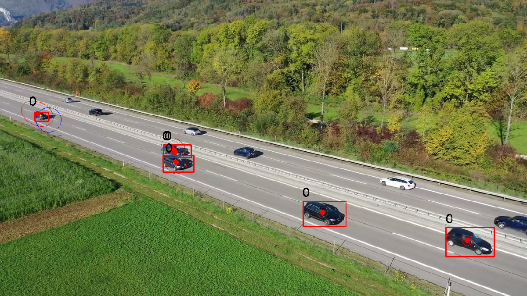
\includegraphics[width=\linewidth]{../../../experiments/E1/V2/DINO/98}
        \caption{Frame number: 98.}
        \label{fig:E1-V2-S3:04}
    \end{subfigure}
    \\
    \begin{subfigure}{0.48\textwidth}
        \centering
        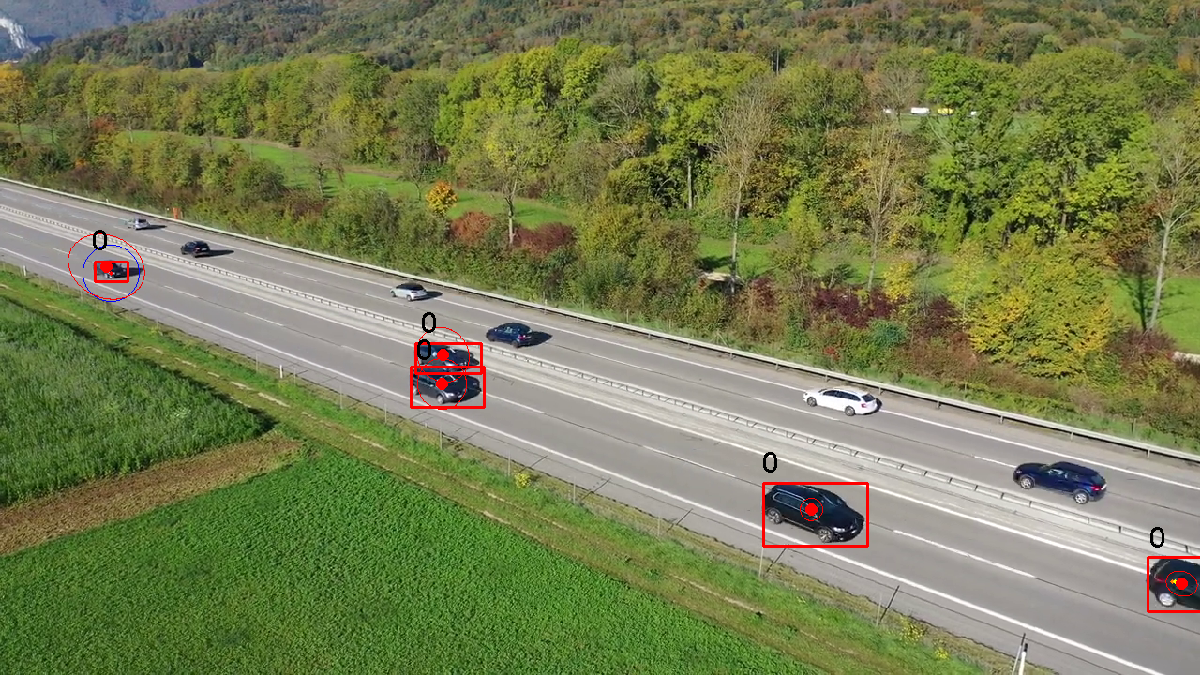
\includegraphics[width=\linewidth]{../../../experiments/E1/V2/DINO/103}
        \caption{Frame number: 103.}
        \label{fig:E1-V2-S3:05}
    \end{subfigure}
    \begin{subfigure}{0.48\textwidth}
        \centering
        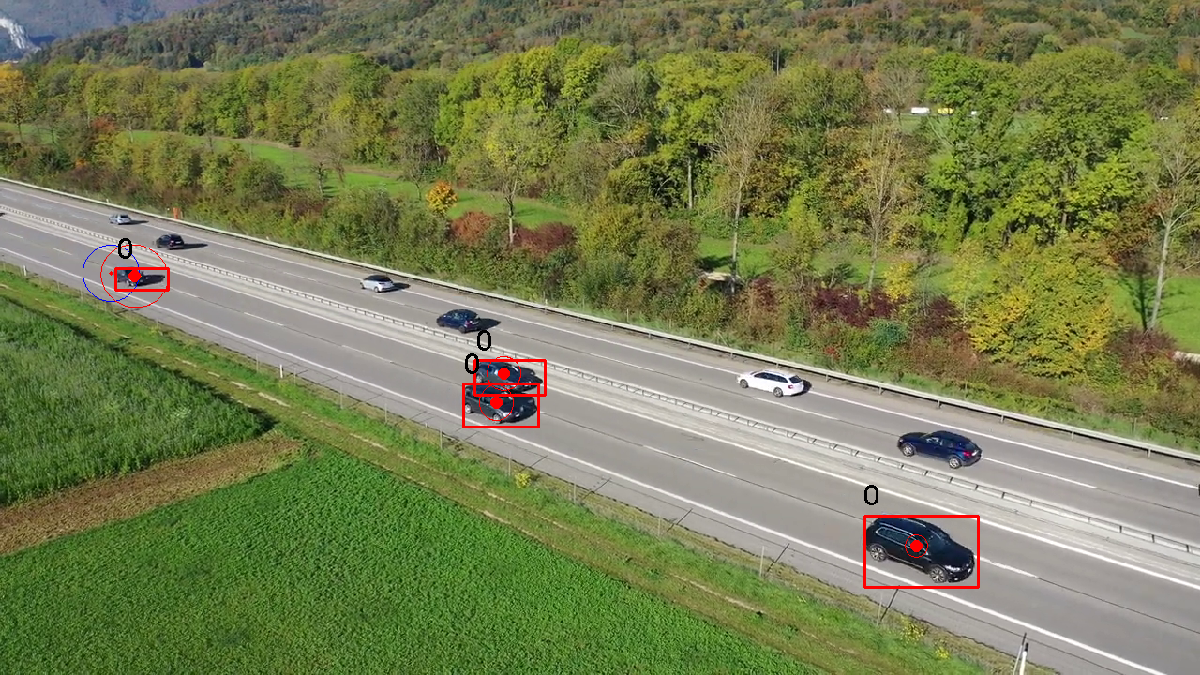
\includegraphics[width=\linewidth]{../../../experiments/E1/V2/DINO/109}
        \caption{Frame number: 109.}
        \label{fig:E1-V2-S3:06}
    \end{subfigure}
    \caption{Image sequence of tracked objects using the GM-PHD filter with the dynamic detection probability, the DINO
    object detector and the SAM image segmentation model.}
    \label{fig:E1-V2-S3}
\end{figure}
